
\documentclass{vgtc}                          % final (conference style)
%\documentclass[review]{vgtc}                 % review
%\documentclass[widereview]{vgtc}             % wide-spaced review
%\documentclass[preprint]{vgtc}               % preprint
%\documentclass[electronic]{vgtc}             % electronic version

%% Uncomment one of the lines above depending on where your paper is
%% in the conference process. ``review'' and ``widereview'' are for review
%% submission, ``preprint'' is for pre-publication, and the final version
%% doesn't use a specific qualifier. Further, ``electronic'' includes
%% hyperreferences for more convenient online viewing.

%% Please use one of the ``review'' options in combination with the
%% assigned online id (see below) ONLY if your paper uses a double blind
%% review process. Some conferences, like IEEE Vis and InfoVis, have NOT
%% in the past.

%% Figures should be in CMYK or Grey scale format, otherwise, colour 
%% shifting may occur during the printing process.

%% These few lines make a distinction between latex and pdflatex calls and they
%% bring in essential packages for graphics and font handling.
%% Note that due to the \DeclareGraphicsExtensions{} call it is no longer necessary
%% to provide the the path and extension of a graphics file:
%% \includegraphics{diamondrule} is completely sufficient.
%%
\ifpdf%                                % if we use pdflatex
  \pdfoutput=1\relax                   % create PDFs from pdfLaTeX
  \pdfcompresslevel=9                  % PDF Compression
  \pdfoptionpdfminorversion=7          % create PDF 1.7
  \ExecuteOptions{pdftex}
  \usepackage{graphicx}                % allow us to embed graphics files
  \DeclareGraphicsExtensions{.pdf,.png,.jpg,.jpeg} % for pdflatex we expect .pdf, .png, or .jpg files
\else%                                 % else we use pure latex
  \ExecuteOptions{dvips}
  \usepackage{graphicx}                % allow us to embed graphics files
  \DeclareGraphicsExtensions{.eps}     % for pure latex we expect eps files
\fi%

%% it is recomended to use ``\autoref{sec:bla}'' instead of ``Fig.~\ref{sec:bla}''
\graphicspath{{figures/}{pictures/}{images/}{./}} % where to search for the images

\usepackage{microtype}                 % use micro-typography (slightly more compact, better to read)
\PassOptionsToPackage{warn}{textcomp}  % to address font issues with \textrightarrow
\usepackage{textcomp}                  % use better special symbols
\usepackage{mathptmx}                  % use matching math font
\usepackage{times}                     % we use Times as the main font
\renewcommand*\ttdefault{txtt}         % a nicer typewriter font
\usepackage{cite}                      % needed to automatically sort the references
\usepackage{tabu}                      % only used for the table example
\usepackage{booktabs}                  % only used for the table example
%% We encourage the use of mathptmx for consistent usage of times font
%% throughout the proceedings. However, if you encounter conflicts
%% with other math-related packages, you may want to disable it.

%% wes 8/2021 additions
\usepackage{comment}    % wes 8/2021
\usepackage{color}      % wes 8/2021
\usepackage{listings}   % wes 8/2021

%% Shun 9/2024 additions
\usepackage{placeins}   % for \FloatBarrier
\usepackage{afterpage} % For \afterpage{\clearpage}
\usepackage{amsmath}
\usepackage[labelfont=bf]{caption} % For make the figure title "Figure 2. " bold
\usepackage{appendix}
\usepackage{graphicx}    % For including graphics
\usepackage{caption}     % For customizing captions
\usepackage{subcaption}  % For creating subfigures
\usepackage{url} 

% wes: for code formatting/coloring
\definecolor{codegreen}{rgb}{0,0.6,0}
\definecolor{codegray}{rgb}{0.5,0.5,0.5}
\definecolor{codepurple}{rgb}{0.58,0,0.82}
\definecolor{backcolour}{rgb}{0.95,0.95,0.92}
\definecolor{codecyan}{rgb}{0.0,0.2,1.0}

% see: https://en.wikibooks.org/wiki/LaTeX/Source_Code_Listings
% set font, size, color style for code listings
\lstdefinestyle{mystyle}{
%    backgroundcolor=\color{backcolour},   
    commentstyle=\textcolor{codegreen},
%    keywordstyle=\color{magenta},    
    keywordstyle=\color{codecyan},
    numberstyle=\tiny\color{codegray},
    stringstyle=\color{codepurple},
    basicstyle=\ttfamily\footnotesize,
    breakatwhitespace=false,    
    breaklines=true,    
    captionpos=b,    
    keepspaces=true,    
    numbers=left,    
    numbersep=2pt,  
    firstnumber=auto,
    numberblanklines=false,
    showspaces=false,
    showstringspaces=false,
    showtabs=false,
    tabsize=2
}
% and then set mystyle to be the default when doing code listings
\lstset{style=mystyle}



%% If you are submitting a paper to a conference for review with a double
%% blind reviewing process, please replace the value ``0'' below with your
%% OnlineID. Otherwise, you may safely leave it at ``0''.
\onlineid{0}

%% declare the category of your paper, only shown in review mode
\vgtccategory{Research}

%% allow for this line if you want the electronic option to work properly
% 8/2021 wes comment out the following line to eliminate build warnings
%\vgtcinsertpkg

%% In preprint mode you may define your own headline.
%\preprinttext{To appear in an IEEE VGTC sponsored conference.}

%% Paper title.

\title{Parallel MMUL and LIKWID Performance Counters \\Assignment \#4, CSC 746, Fall 2024}

%% This is how authors are specified in the conference style

%% Author and Affiliation (single author).
%%\author{Roy G. Biv\thanks{e-mail: roy.g.biv@aol.com}}
%%\affiliation{\scriptsize Allied Widgets Research}

%% Author and Affiliation (multiple authors with single affiliations).
%%\author{Roy G. Biv\thanks{e-mail: roy.g.biv@aol.com} %
%%\and Ed Grimley\thanks{e-mail:ed.grimley@aol.com} %
%%\and Martha Stewart\thanks{e-mail:martha.stewart@marthastewart.com}}
%%\affiliation{\scriptsize Martha Stewart Enterprises \\ Microsoft Research}

%% Author and Affiliation (multiple authors with multiple affiliations)
\author{Shun Usami\thanks{email:susami@sfsu.edu}\\ %
        \scriptsize SFSU}

%% A teaser figure can be included as follows, but is not recommended since
%% the space is now taken up by a full width abstract.
%\teaser{
%  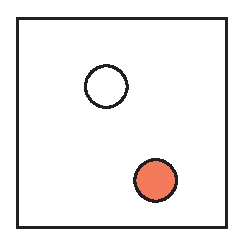
\includegraphics[width=1.5in]{sample.eps}
%  \caption{Lookit! Lookit!}
%}

%% Abstract section.
\abstract{
% Please take a few moments and try to compose an abstract for your homework writeup. It should contain these ideas: what was the problem being studied, what was the approach (what did you implement), what are the results.
% The abstract should describe the basic message of the paper, including: the problem, why your solution should be of interest, some notion that your solution is effective, and a teaser about how it has been evaluated. Cover all of this using between 75 and 150 words. Thus, the abstract is the hardest part to write. Sometimes I try to write it first, but the final version is usually composed of items drawn from the introduction, and then condensed, as the last step of writing the paper.

% describes the focus of the study, the approach, and the primary findings/results (3 or 4 sentences total). Writing tip: it's often the case that the Abstract and Introduction are the last items written in a technical paper, once you know the outcome of the performance study.

This assignment investigates two performance optimization techniques—parallelism and cache utilization—by evaluating the performance of three matrix multiplication (MM) methods: Basic Matrix Multiplication with OpenMP (Basic OMP), Blocked Matrix Multiply with Copy Optimization (BMMCO OMP), and CBLAS, using hardware counters. The implementations were tested across varying matrix sizes (\(128 \times 128\), \(512 \times 512\), and \(2048 \times 2048\)) and thread counts (1, 4, 16, and 64) to assess speedup and efficiency. Results indicate that while Basic OMP scales effectively with increasing thread count, BMMCO OMP exhibits limited scalability for smaller matrices and larger block sizes due to thread underutilization. The BMMCO OMP method significantly reduced L2 and L3 cache accesses, particularly with larger block sizes, resulting in superior performance compared to Basic OMP. These findings suggest that achieving optimal performance requires balancing between increasing cache utilization through larger block sizes and maximizing thread utilization with smaller block sizes.
} % end of abstract

%% ACM Computing Classification System (CCS). 
%% See <http://www.acm.org/class/1998/> for details.
%% The ``\CCScat'' command takes four arguments.

% not needed for CSC 746 Fall 2021
%\CCScatlist{ 
%  \CCScat{K.6.1}{Management of Computing and Information Systems}%
%{Project and People Management}{Life Cycle};
%  \CCScat{K.7.m}{The Computing Profession}{Miscellaneous}{Ethics}
%}

%% Copyright space is enabled by default as required by guidelines.
%% It is disabled by the 'review' option or via the following command:
% \nocopyrightspace

%%%%%%%%%%%%%%%%%%%%%%%%%%%%%%%%%%%%%%%%%%%%%%%%%%%%%%%%%%%%%%%%
%%%%%%%%%%%%%%%%%%%%%% START OF THE PAPER %%%%%%%%%%%%%%%%%%%%%%
%%%%%%%%%%%%%%%%%%%%%%%%%%%%%%%%%%%%%%%%%%%%%%%%%%%%%%%%%%%%%%%%%

\begin{document}

%% The ``\maketitle'' command must be the first command after the
%% ``\begin{document}'' command. It prepares and prints the title block.

%% the only exception to this rule is the \firstsection command
%\firstsection{Introduction}

\maketitle
\[
C = C + A \times B
\]

\[
C_{ij} = C_{ij} + \sum_{k=1}^{n} A_{ik} \times B_{kj}
\]

Where:
\begin{itemize}
    \item \( A \) is an \( n \times n \) matrix.
    \item \( B \) is an \( n \times n \) matrix.
    \item \( C \) is an \( n \times n \) matrix.
    \item \( i \), \( j \), and \( k \) are the indices of the matrix elements.
\end{itemize}
\section{Introduction}
% consists of 3 short paragraphs consisting of the problem statement, your approach, and a brief summary of the findings/results. Here, short paragraph means 3-4 sentences.

The objective of this study is to evaluate the effectiveness of different parallelization techniques for enhancing computational efficiency and memory bandwidth utilization in matrix-vector multiplication (VMM). The techniques explored include instruction-level parallelism, SIMD instructions, vectorization, multi-threading with OpenMP, and considerations for NUMA architecture. By examining these methods, we aim to understand their respective benefits and limitations in the context of high-performance computing.

We implemented four versions of VMM: a basic serial version as an unoptimized baseline, a highly optimized serial version using the CBLAS library, an automatically vectorized serial version leveraging SIMD instructions, and a parallel version utilizing OpenMP for multi-threading. These implementations provide a comprehensive basis for evaluating the impact of different optimizations on performance. All experiments were conducted on the Perlmutter supercomputer at NERSC, using C++ for implementation. Detailed descriptions of these methods are provided in Section~\ref{sec:methodology}.

The results indicate that the Vectorized implementation achieved four times the performance of the Basic version due to SIMD instructions and performed similarly to CBLAS for larger matrix sizes. However, CBLAS significantly outperformed the Vectorized version for smaller matrices, likely due to techniques like instruction-level parallelism (ILP). The OpenMP implementation, while outperforming CBLAS for larger matrices, had excessive overhead for smaller sizes, making it worse than both CBLAS and even the Vectorized version. Despite outperforming CBLAS for larger sizes, the OpenMP performance was still far from ideal due to memory data layout inefficiencies and limited bandwidth, which acted as bottlenecks.
% For homework writeups, the Introduction section should state the general thrust of the assignment.

% What is the problem being studied? Explain in 2-3 sentences.

% What is the approach for studying the problem? Hint: the approach consists of the program(s) you are writing, so say in 2-3 sentences something about those programs. If you like, it is ok to use a forward reference, and say something like "we present the implementation in \S\ref{sec:implementation}. 

% What are the main results? Say something about the results in 2-3 sentences: what is the nature of your experiment that tests your implementation, and say something about the insights gained. 

\begin{comment}
%% the material that follows is from the generic tech paper skeleton project

The problem we have solved
\begin{itemize}
    \item Concentrate on making this assertion and only this assertion in a succinct set of 1 to 3 paragraphs
    \item A common mistake is to explain too much of the problem context first. Instead, state the problem essentially as a claim, and leave explanations supporting your claim to the next part, “Why it is not already solved.”
\end{itemize}

Why the problem is not already solved or other solutions are ineffective in one or more important ways
\begin{itemize}

\item Your new idea need not solve every problem but it should solve at least one that is not already solved
\item This is the place to provide a succinct description of the problem context giving enough information to support the claim that a problem exists, made in the preceding problem declaration.
  
\end{itemize}

Why our solution is worth considering and why is it effective in some way that others are not

\begin{itemize}
\item A succinct statement of why the reader should care enough to read the rest of the paper.
\item This should include a statement about the characteristics of your solution to the problem which 1) make it a solution, and 2) make it superior to other solutions to the same problem.
\end{itemize}

How the rest of the paper is structured
\begin{itemize}
    \item The short statement below is often all you need, but you should change it when your paper has a different structure, or when more information is required to describe what a given section contains. If it isn’t required then you don’t want to say it here.
\end{itemize}

The rest of this paper first discusses related work in Section 2, and then describes our implementation in Section 3. Section 4 describes how we evaluated our system and presents the results. Section 5 presents our conclusions and describes future work.

\end{comment}

% Put an introductory paragraph here that gives the reader an overview of what's coming. If there are multiple subsections, say in a few words or a sentence something about each subsection.

% include a separate subsection for each of the different implementations. Briefly describe your implementation, and include the use of compact pseudocode as necessary. The focus here should be on conciseness and clarity. Be sure to describe the strategy you used in parallelizing your code. Your example Listings should clearly indicate the OpenMP pragmas you used. 

This section presents three MM implementations aimed at evaluating performance improvements through parallelization and optimization techniques. The first implementation, Basic OMP, evaluates the impact of adding shared-memory parallelism to a simple MM approach. The second, Blocked Matrix Multiplication with Copy Optimization (BMMCO), combines cache optimization techniques with parallelization to further enhance computational efficiency. Finally, the CBLAS MM serves as a baseline, using a highly optimized but serial implementation.

Each subsection details the objectives, describes the applied techniques, and presents compact pseudocode or listings to illustrate the use of OpenMP and optimization strategies.

\subsection{Overall Code Harnesss}
\label{subsec:overall-code-harness}
% Using Listings where appropriate to present your code ideas, as well as describe these ideas in text form. Each of these subsections should consist of 2-3 short paragraphs of 4-5 sentences each (hint: explain the problem you’re trying to solve, and how you solve it in your code, and the relationship of the code in this subsection to the rest of the larger problem).

% Describe the implementation (2-3 sentences, or more if needed).
Listing~\ref{listing:overall-code-harness} presents the structure of the distributed-memory stencil operation. Each process computes the mesh decomposition independently to determine how the computational domain is divided among the available ranks. The host process (rank 0) reads the input file and distributes the corresponding data segments (tiles) to all ranks using a scatter operation. Each rank then applies the Sobel filter to its assigned tiles, ensuring an even distribution of computational workload. After processing, the results are sent back to the host process via a gather operation. Finally, the host aggregates the data and writes the output file.

\begin{lstlisting}[caption={\textbf{Overall code harness of the distributed-memory stencil operations with MPI.}},label={listing:overall-code-harness},float=htbp,style=mystyle,language=C++]
int main(int argc, char *argv[]) {
    MPI_Init(&argc, &argv);
    parseArgs();
    computeMeshDecomposition();
    loadInputFile();   // Only Rank 0 loads 
    scatterAllTiles(); // Rank 0 sends, the others receive
    sobelAllTiles();
    gatherAllTiles();  // Rank 0 receives, the others send
    writeOutputFile(); // Only Rank 0 writes
    MPI_Finalize();
    return 0;
}
\end{lstlisting}
\FloatBarrier

\subsection{Decomposition Strategies}
\label{subsec:decomposition-strategies}
To parallelize the Sobel filter, we implemented three decomposition methods to divide the computational domain among MPI ranks:
\begin{itemize}
    \item \textbf{Row-slab Decomposition:} The input image is divided horizontally into row-wise slabs, and each rank processes one row.
    \item \textbf{Column-slab Decomposition:} The input image is divided vertically into column-wise slabs, and each rank processes one column.
    \item \textbf{Tiled Decomposition:} The input image is divided into smaller rectangular tiles, where each rank processes one tile.
\end{itemize}

Figure~\ref{fig:decomposition-methods} illustrates these decomposition methods using a total of 16 ranks.

\begin{figure}[h]
    \centering
    \begin{subfigure}{0.3\textwidth}
        \centering
        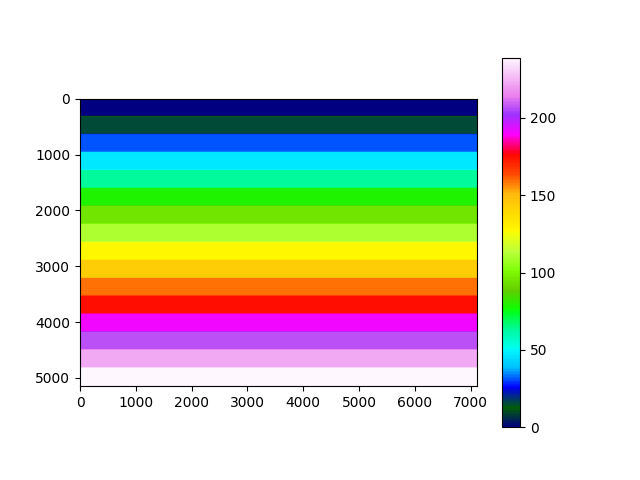
\includegraphics[width=\textwidth]{images/row_slab.png}
        \caption{Row-slab Decomposition}
        \label{fig:row-slab}
    \end{subfigure}
    \hfill
    \begin{subfigure}{0.3\textwidth}
        \centering
        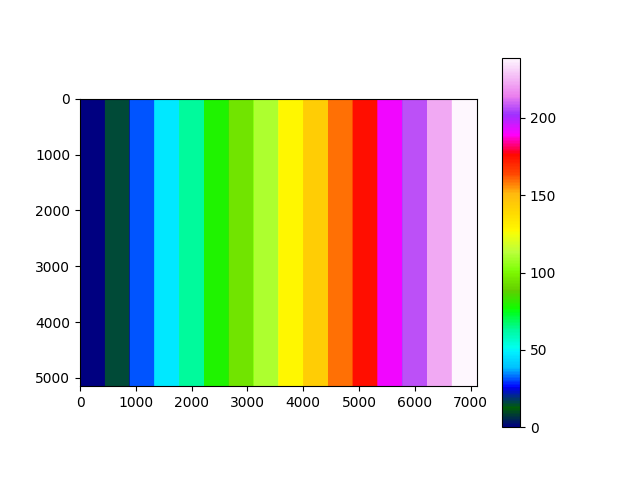
\includegraphics[width=\textwidth]{images/column_slab.png}
        \caption{Column-slab Decomposition}
        \label{fig:column-slab}
    \end{subfigure}
    \hfill
    \begin{subfigure}{0.3\textwidth}
        \centering
        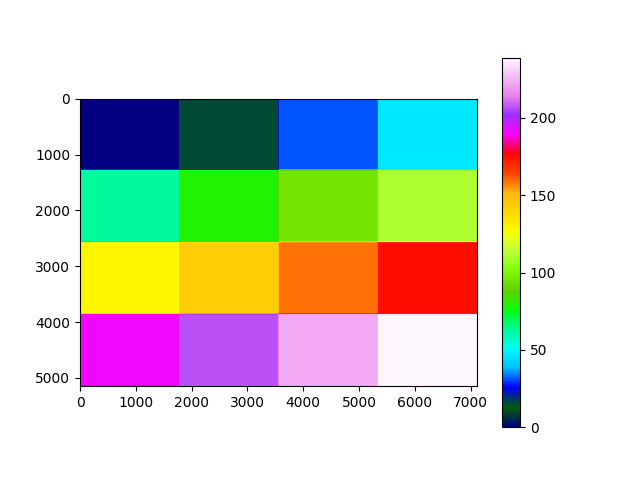
\includegraphics[width=\textwidth]{images/tiled.png}
        \caption{Tiled Decomposition}
        \label{fig:tiled}
    \end{subfigure}
    \caption{Graphical representation of the decomposition strategies (Row-slab, Column-slab, and Tiled) using a total of 16 ranks.}
    \label{fig:decomposition-methods}
\end{figure}
\FloatBarrier

\subsection{Handling Halo cells}
\label{subsec:handling-halo-cells}

Proper handling of tile boundaries is crucial to ensure the accuracy of our Sobel computation. As depicted in Figure~\ref{fig:tile-boundary}, neglecting to process tile boundaries appropriately results in assigning a value of 0.0 to pixels along the shared tile edges. 

To address this issue, halo cells are incorporated into the computation. During the scatter phase, halo cells are sent along with the data tiles. These halo cells are then utilized during the Sobel processing phase to ensure seamless computation across tile boundaries. It is important to note that halo cells are not transmitted back during the gathering phase.

\begin{figure}[h!]
    \centering
    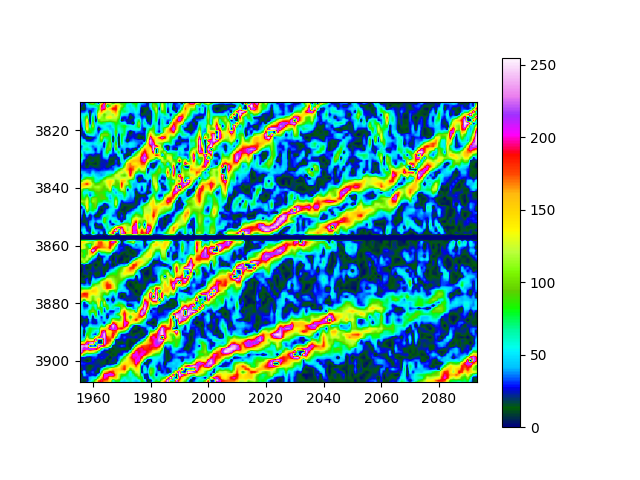
\includegraphics[width=\linewidth]{images/tile-boundary.png}
    \caption{Illustration of tile boundaries without appropriate halo cell processing.}
    \label{fig:tile-boundary}
\end{figure}
\FloatBarrier

\subsection{Send and Receive Strided Buffer}
\label{subsec:send-and-receive-strided-buffer}

% State the objective for the implementation (2-3 sentences).
The \textit{sendStridedBuffer} and \textit{recvStridedBuffer} functions are designed to efficiently facilitate data exchange between MPI ranks, particularly for handling non-contiguous memory regions. These functions are crucial for two key operations: scattering input image data from rank zero to non-zero ranks and gathering computed results from non-zero ranks back to rank zero.

\subsubsection{Send Strided Buffer}
\label{subsubsec:send-strided-buffer}

% Describe the implementation (2-3 sentences, or more if needed).
The \textit{sendStridedBuffer} function facilitates the transmission of a subregion from a source buffer (\textit{srcBuf}) on one MPI rank (\textit{fromRank}) to another (\textit{toRank}). As illustrated in Listing~\ref{listing:send-strided-buffer}, this function uses \textit{MPI\_Type\_create\_subarray()} to define a subarray datatype. This datatype specifies the full buffer dimensions, the size of the subregion (\textit{sendWidth} by \textit{sendHeight}), and the offset of the subregion within the buffer (\textit{srcOffsetColumn}, \textit{srcOffsetRow}). By encapsulating the data representation into a single MPI datatype, the function eliminates the need for intermediate buffers, manual data packing, or multiple \textit{MPI\_Send()} calls.

\begin{lstlisting}[caption={\textbf{Implementation of the send strided buffer function.}},label={listing:send-strided-buffer},float=htbp,style=mystyle,language=C++]

void sendStridedBuffer(float *srcBuf, int srcWidth, int srcHeight, int srcOffsetColumn, int srcOffsetRow, int sendWidth, int sendHeight, int fromRank, int toRank) {
  int msgTag = 0;

  // Create the subarray datatype
  MPI_Datatype subarray_type;
  int dimensions_full_array[2] = {srcHeight, srcWidth};
  int dimensions_subarray[2] = {sendHeight, sendWidth};
  int start_coordinates[2] = {srcOffsetRow, srcOffsetColumn};
  MPI_Type_create_subarray(2, dimensions_full_array, dimensions_subarray, start_coordinates, MPI_ORDER_C, MPI_FLOAT, &subarray_type);
  MPI_Type_commit(&subarray_type);

  // Send the message
  int count = 1;
  MPI_Send(srcBuf, count, subarray_type, toRank, msgTag, MPI_COMM_WORLD);

  // Free the datatype
  MPI_Type_free(&subarray_type);
}

\end{lstlisting}
\FloatBarrier

\subsubsection{Receive Strided Buffer}
\label{subsubsec:receive-strided-buffer}

% Describe the implementation (2-3 sentences, or more if needed).
The \textit{recvStridedBuffer} function receives a subregion of data into a destination buffer (\textit{dstBuf}) from one MPI rank (\textit{fromRank}) to another (\textit{toRank}). As shown in Listing~\ref{listing:receive-strided-buffer} and similar to the \textit{sendStridedBuffer} function described in Section~\ref{subsubsec:send-strided-buffer}, it uses a custom subarray MPI datatype to define the dimensions and offset of the subregion within the larger buffer. This ensures efficient placement of the received data directly into the appropriate non-contiguous memory region.

\begin{lstlisting}[caption={\textbf{Implementation of the receive strided buffer function.}},label={listing:receive-strided-buffer},float=htbp,style=mystyle,language=C++]
void recvStridedBuffer(float *dstBuf, int dstWidth, int dstHeight, int dstOffsetColumn, int dstOffsetRow, int expectedWidth, int expectedHeight, int fromRank, int toRank) {
  int msgTag = 0;
  MPI_Status stat;

  // Create the subarray datatype
  MPI_Datatype subarray_type;
  int dimensions_full_array[2] = {dstHeight, dstWidth};
  int dimensions_subarray[2] = {expectedHeight, expectedWidth};
  int start_coordinates[2] = {dstOffsetRow, dstOffsetColumn};
  MPI_Type_create_subarray(2, dimensions_full_array, dimensions_subarray, start_coordinates, MPI_ORDER_C, MPI_FLOAT, &subarray_type);
  MPI_Type_commit(&subarray_type);

  // Receive the message
  int count = 1;
  MPI_Recv(dstBuf, count, subarray_type, fromRank, msgTag, MPI_COMM_WORLD, &stat);

  // Free the datatype
  MPI_Type_free(&subarray_type);
}
\end{lstlisting}

\FloatBarrier

\subsection{Sobel Implementation}
\label{subsec:sobel-implementation}

\subsubsection{Sobel Operator}
\label{subsubsec:sobel-operator}

The Sobel operator approximates the gradient of image intensity for edge detection~\cite{kanopoulos1988design}. It uses two \(3 \times 3\) kernels, convolved with the original image \( A \), to compute horizontal and vertical gradients \( G_x \) and \( G_y \):

\[
G_x = \begin{bmatrix}
+1 & 0 & -1 \\
+2 & 0 & -2 \\
+1 & 0 & -1 \\
\end{bmatrix} * A,
\quad
G_y = \begin{bmatrix}
+1 & +2 & +1 \\
0  &  0 &  0 \\
-1 & -2 & -1 \\
\end{bmatrix} * A
\]

The gradient magnitude at each pixel is computed as:

\[
G = \sqrt{G_x^2 + G_y^2}
\]

The function \texttt{sobel\_filtered\_pixel()} computes the Sobel filter at a pixel location, as shown in Listing~\ref{listing:sobel-filtered-pixel}. The arrays \( gx \) and \( gy \) represent the kernel weights for the horizontal and vertical filters, respectively.

\begin{lstlisting}[caption={\textbf{Sobel filtered pixel computation.} Computes the Sobel filter at a specific pixel location.},label={listing:sobel-filtered-pixel},float=htbp,style=mystyle,language=C++]
Function sobel_filtered_pixel(img[width, height], x, y, gx[3, 3], gy[3, 3]) {
    if x or y is at the boundary of the img
        return 0
    Gx = 0.0, Gy = 0.0;
    for j in {0, 1, 2}
        for i in {0, 1, 2}
            xx = x - 1 + i;
            yy = y - 1 + j;
            Gx += img[xx, yy] * gx[i, j];
            Gy += img[xx, yy] * gy[i, j];
    return sqrt(Gx * Gx + Gy * Gy);
}
\end{lstlisting}

\FloatBarrier
\subsubsection{Overall Sobel Filtering}
The implementation of \texttt{do\_sobel\_filtering()} function is shown in Listing~\ref{listing:sobel-implementation}, which applies the Sobel filter to a specified region of an input buffer (\texttt{in}) and stores the processed output in a designated output buffer (\texttt{out}). This function processes each pixel in the region by invoking the \texttt{sobel\_filtered\_pixel()} function (detailed in Listing~\ref{listing:sobel-filtered-pixel}), which calculates the gradient magnitude for the pixel using the Sobel operator. The computed values are then placed into their corresponding positions in the output buffer. Each rank independently calls \texttt{do\_sobel\_filtering()} to compute the filtered output for its assigned tile, ensuring parallel processing across the distributed tiles.

\begin{lstlisting}[caption={\textbf{Implementation of the Sobel operation for a given region.}},label={listing:sobel-implementation},float=htbp,style=mystyle,language=C++]
void do_sobel_filtering(float *in, float *out, int width, int height) {
  // Define Sobel operator kernels
  float Gx[] = {1.0, 0.0, -1.0, 2.0, 0.0, -2.0, 1.0, 0.0, -1.0};
  float Gy[] = {1.0, 2.0, 1.0, 0.0, 0.0, 0.0, -1.0, -2.0, -1.0};
  
  // Apply Sobel filtering to each pixel
  for (int y = 0; y < height; ++y) {
    for (int x = 0; x < width; ++x) {
      // Compute the Sobel-filtered value for the current pixel
      out[y * width + x] =
          sobel_filtered_pixel(in, x, y, width, height, Gx, Gy);
    }
  }
}
\end{lstlisting}
\FloatBarrier
\section{Results}
% Provide an introductory paragraph that summarizes what's in this section: a list of runs/experiments intended to test your implementation and ideas. Describe each of these experiments in a few words/a sentence.

In this section, we analyze how our distributed-memory implementation of the Sobel filter improves computational efficiency by leveraging parallel execution across multiple CPU nodes. We evaluate the performance of three grid decomposition strategies—Column-slab, Row-slab, and Tiled—under various concurrency levels. We start by describing the computational platform and software environment we used for our experiments. Next, we explain our methodology, including decomposition techniques, runtime measurement, data movement tracking, and speedups to assess parallel performance. Through our runtime performance and data movement studies, we identify how task distribution, communication, and synchronization influence overall efficiency. Finally, we discuss our findings and suggest optimizations to enhance scalability and performance accuracy.

% What machine did you run your tests on? What was the processor, its clock rate (GHz), size of L1/L2/L3 cache, how much memory (DRAM), what OS?

% What compiler did you use, what compilation flags?

% Include a subsection describing your computational platform and software environment. Please add a citation to the location where you found this information (hint: use the LaTeX \cite{} command, and add a new entry to the template.bib file provided with the Overleaf template).

The experiments were conducted on a CPU node of the Perlmutter supercomputer at NERSC. Each node is equipped with two AMD EPYC 7763 (Milan) processors, each featuring 64 cores running at a clock rate of 2.45 GHz. These cores support Simultaneous Multi-threading (SMT), enabling two threads per core. Each core has 32 KiB of L1 cache and 512 KiB of L2 cache, while 8 cores share a 32 MiB L3 cache. The AMD EPYC 7763 processor also features 8 memory channels per socket, with 2 DIMMs per channel, and 4 NUMA domains per socket (NPS=4) \cite{amd_epyc_tuning_guide}.

The system is supported by 512 GiB of DDR4 DRAM, offering a memory bandwidth of 204.8 GiB/s per CPU. The processors utilize the AVX2 instruction set for vector processing, and each core has a peak computational throughput of 39.2 GFLOPS \cite{nersc_perlmutter_architecture}.

All experiments were conducted on a single CPU node running \textit{SUSE Linux Enterprise Server 15 SP4}, with kernel version \textit{5.14.21-150400.24.81\_12.0.87-cray\_shasta\_c} \cite{usami2024hostnamectl}. The C++ code was compiled using \textit{g++-12 (SUSE Linux) 12.3.0} with the following optimization flags: \texttt{-fopenmp -Wall -pedantic -march=native}. Note that the \texttt{-fopenmp} flag was not used for compiling the CBLAS implementation.

The following OpenMP environmental variables were used for the VMM OpenMP implementation. The variable \texttt{OMP\_NUM\_THREADS} was left unset as it conflicts with \texttt{likwid-perfctr} on Perlmutter:
\begin{itemize}
    \item \texttt{OMP\_PLACES=threads}: Assigns each OpenMP thread to a separate hardware thread, ensuring efficient mapping to processing units.
    \item \texttt{OMP\_PROC\_BIND=spread}: Distributes threads evenly across the available CPUs, aiming for optimal workload balancing.
\end{itemize}

The execution command for each program was:
\begin{quote}
\texttt{likwid-perfctr -m -g FLOPS\_DP -C N:0-\${num\_threads-1} ./benchmark -N \$N}
\end{quote}

The command runs the benchmark executable while collecting performance metrics using \texttt{likwid-perfctr}. The options used in the command are as follows:
\begin{itemize}
    \item \texttt{-g FLOPS\_DP}: Specifies the performance group to measure, in this case, the \textit{FLOPS\_DP} group, which tracks double-precision floating-point operations to evaluate computational throughput.
    \item \texttt{-C N:0-\${num\_threads-1}}: Binds the execution to a set of cores. The option \texttt{N:0-\${num\_threads-1}} allows specification of core IDs from 0 to \texttt{num\_threads-1}, where \texttt{num\_threads} represents the nuMiBer of threads being used. This ensures that only the desired cores are used during the run.
\end{itemize}
% What machine did you run your tests on? What was the processor, its clock rate (GHz), size of L1/L2/L3 cache, how much memory (DRAM), what OS?

% What compiler did you use, what compilation flags?


\subsection{Methodology}
\label{subsec:methodology}

\subsubsection{Problem Sizes and Concurrency Levels}
\label{subsubsec:problem-size}
To evaluate the Sobel filter implementations, we tested a fixed grayscale image with dimensions \(7112 \times 5146\). Experiments were conducted using three decomposition methods: Row-slab, Column-slab, and Tiled. For each method, we analyzed performance across varying total ranks: 4, 9, 16, 25, 36, 49, 64, and 81, capturing the impact of concurrency on runtime.

\subsubsection{Runtime Measurement}
\label{subsubsec:runtime}
Performance data was collected by measuring the runtime of three key phases: Scatter, Sobel computation, and Gather. Timing was performed on the CPU using the C++ \texttt{chrono\_timer()}, which encapsulated the \texttt{scatterAllTiles}, \texttt{sobelAllTiles}, and \texttt{gatherAllTiles} functions, respectively. 

To ensure accurate synchronization across all ranks, \texttt{MPI\_Barrier} was employed before starting and stopping timers for each phase. This approach guarantees that all ranks finish the preceding phase before advancing to the next, thereby isolating the runtime measurements for each phase and avoiding overlap between operations.

\subsubsection{Data Movement}
\label{subsubsec:data-movement}
The number of messages and total data size were measured by implementing counters before calling \texttt{MPI\_Send} and calculating the data size using \texttt{MPI\_Type\_size}. These values were aggregated using \texttt{MPI\_Reduce} to provide a global summary.

\subsubsection{Speedup Calculation}
\label{subsubsec:speedup}
Speedup was derived from the runtime data to evaluate the parallel performance of the Sobel filter implementations. The speedup \(S(n, p)\) is defined as:

\begin{displaymath}
    S(n, p) = \frac{T^*(n)}{T(n, p)}
\end{displaymath}

Here, \(T^*(n)\) is the runtime of the best sequential algorithm for a problem of size \(n\), measured as the runtime with a single process per CPU node (total ranks of 4). \(T(n, p)\) represents the runtime for the same problem size \(n\) using \(p\) parallel threads. Since the problem size was fixed (\(7112 \times 5146\) image), the variability in \(p\) allowed us to assess the scalability of each decomposition method.

\subsection{Runtime Performance Study}
\label{subsec:runtime-performance-study}
\begin{figure}[htbp]
    \centering
    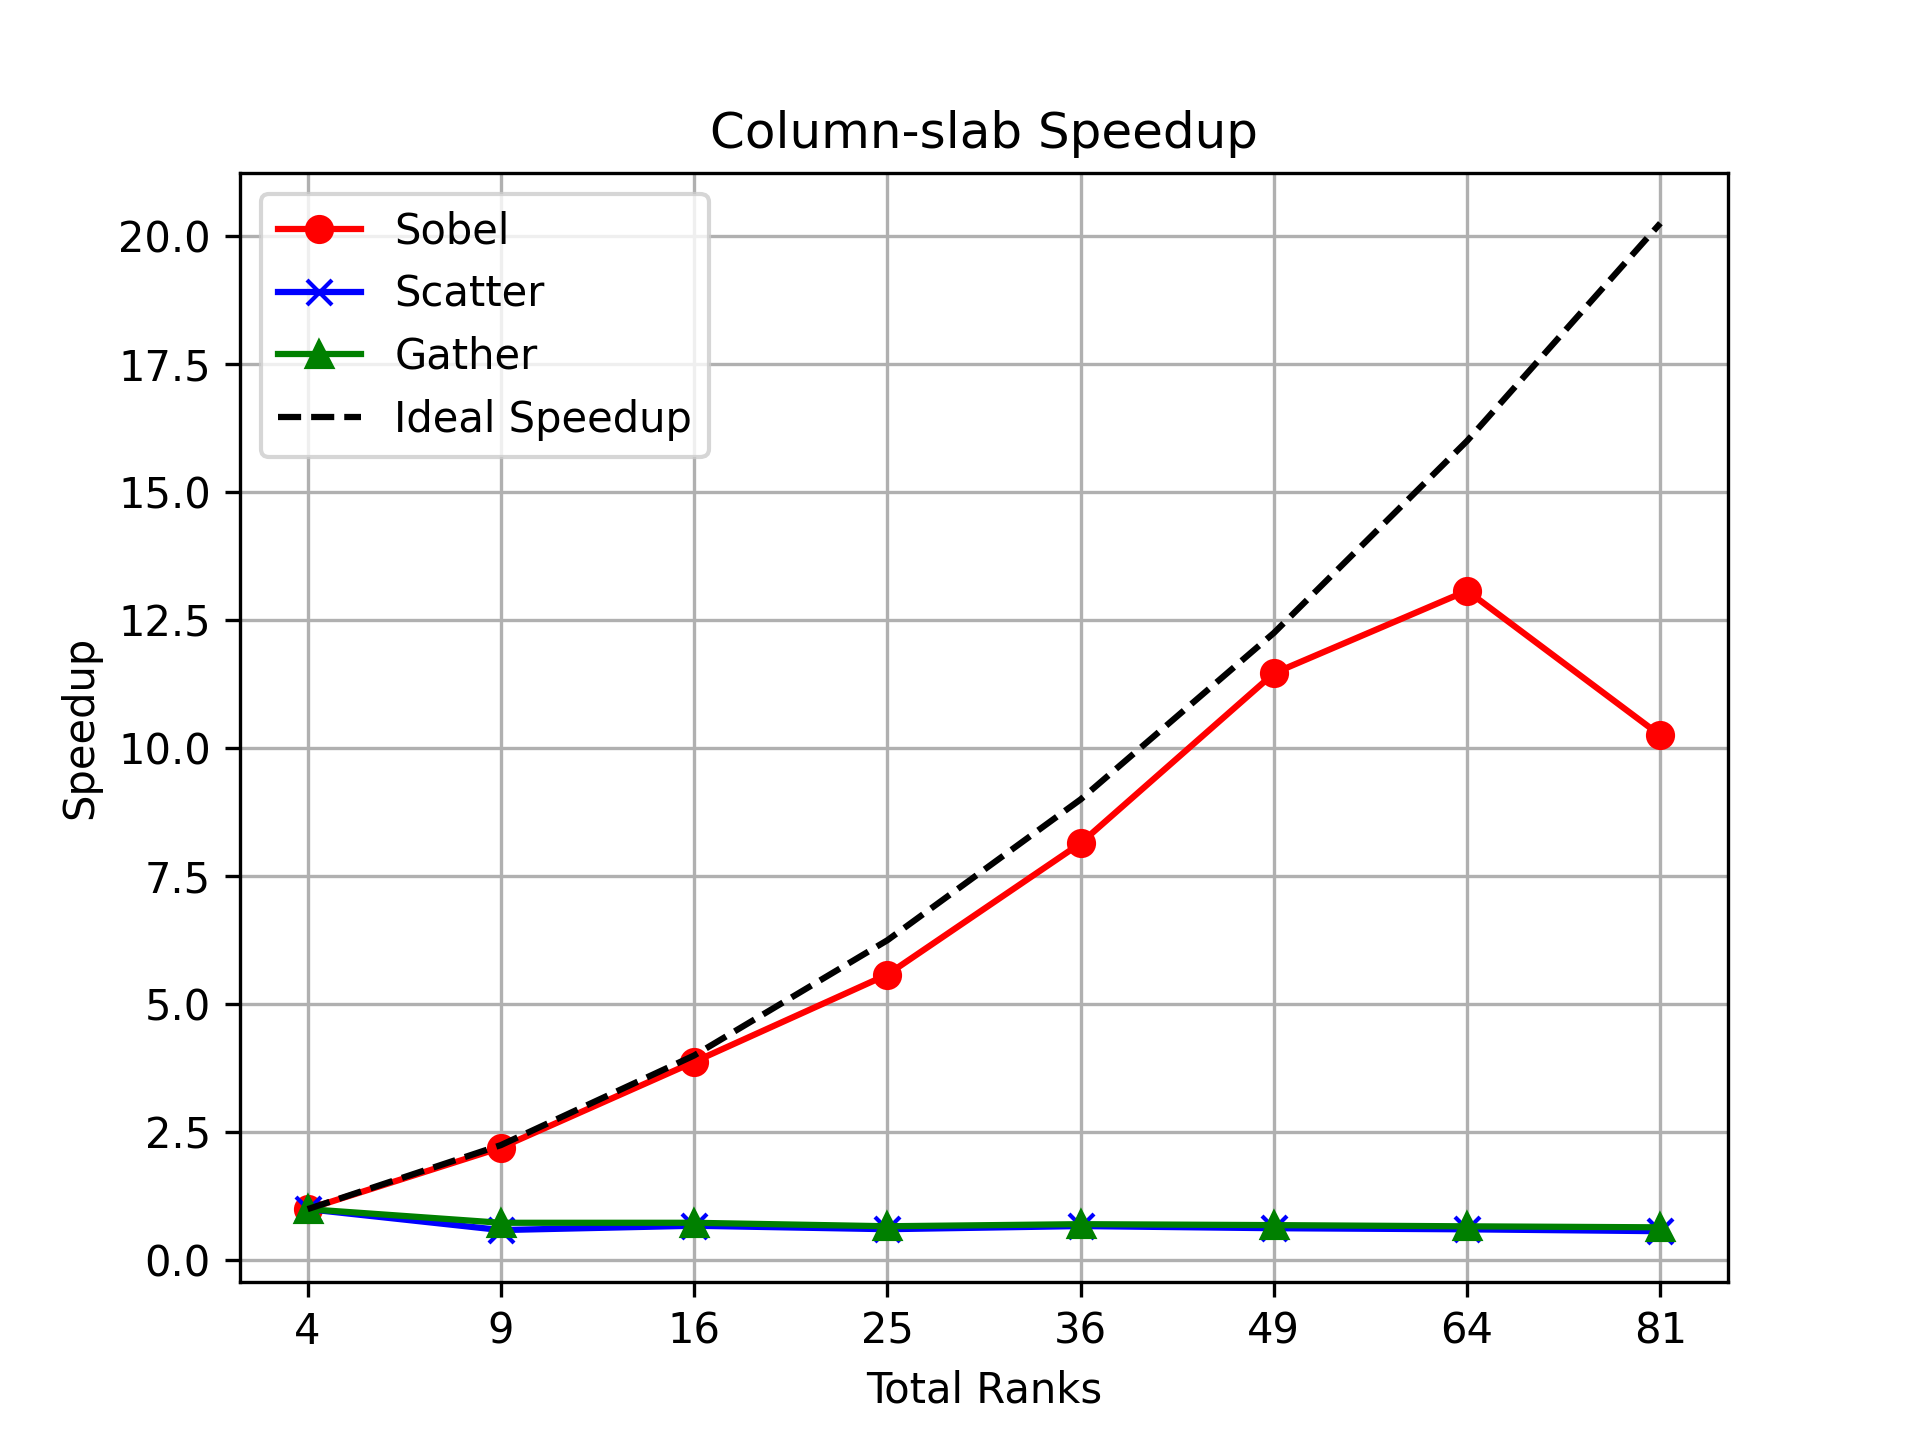
\includegraphics[width=1.0\linewidth]{images/column-slab_speedup.png}
    \caption{Speedup chart for Column-slab decomposition.}
    \label{fig:speedup-column}
\end{figure}

\begin{figure}[htbp]
    \centering
    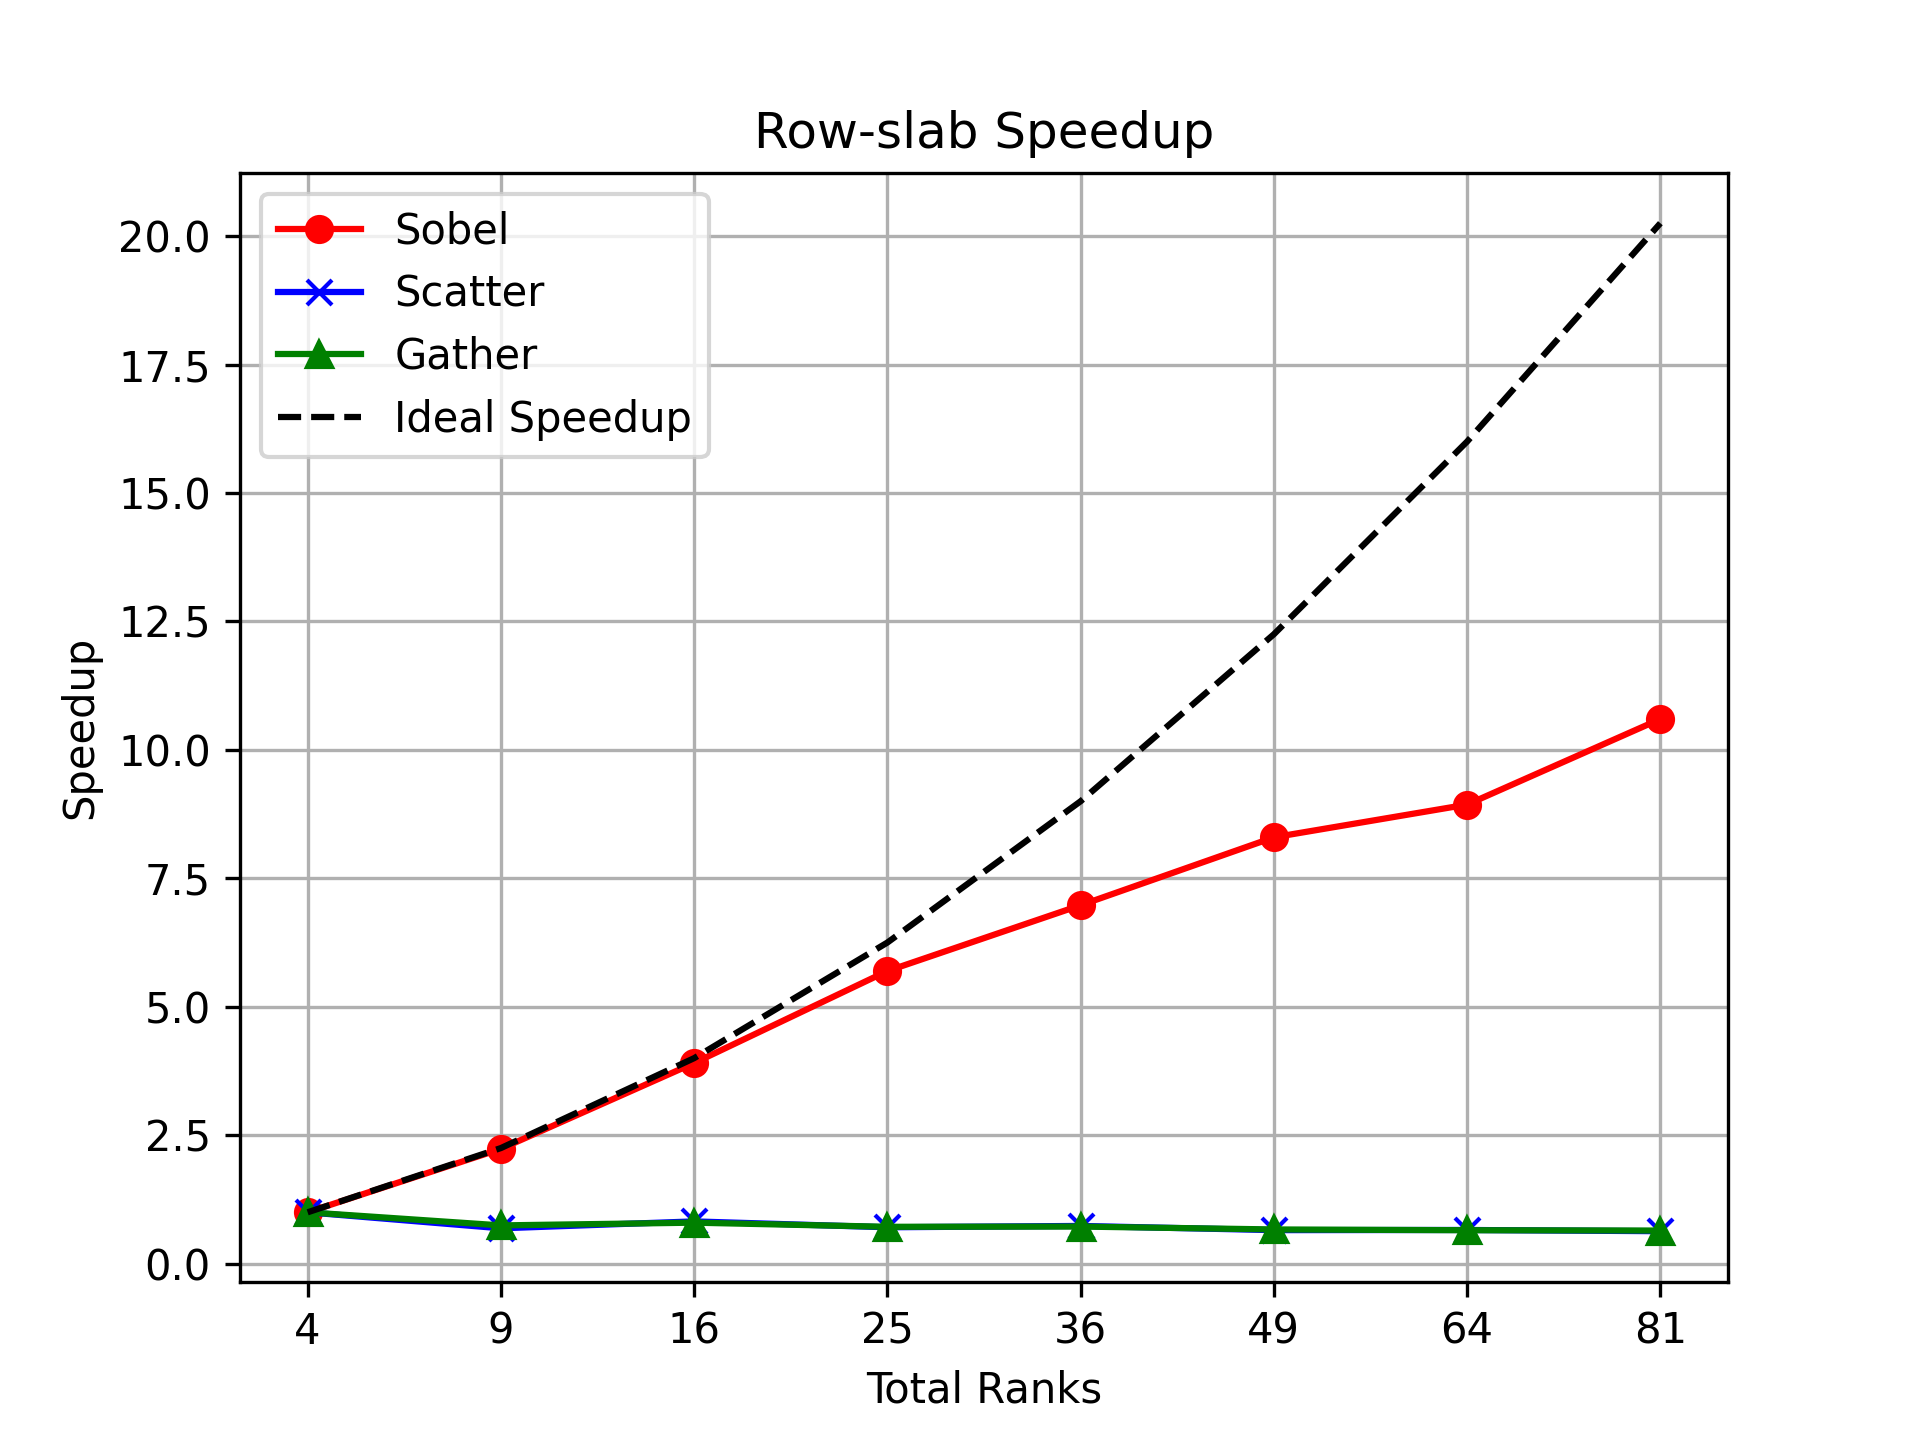
\includegraphics[width=1.0\linewidth]{images/row-slab_speedup.png}
    \caption{Speedup chart for Row-slab decomposition.}
    \label{fig:speedup-row}
\end{figure}

\begin{figure}[htbp]
    \centering
    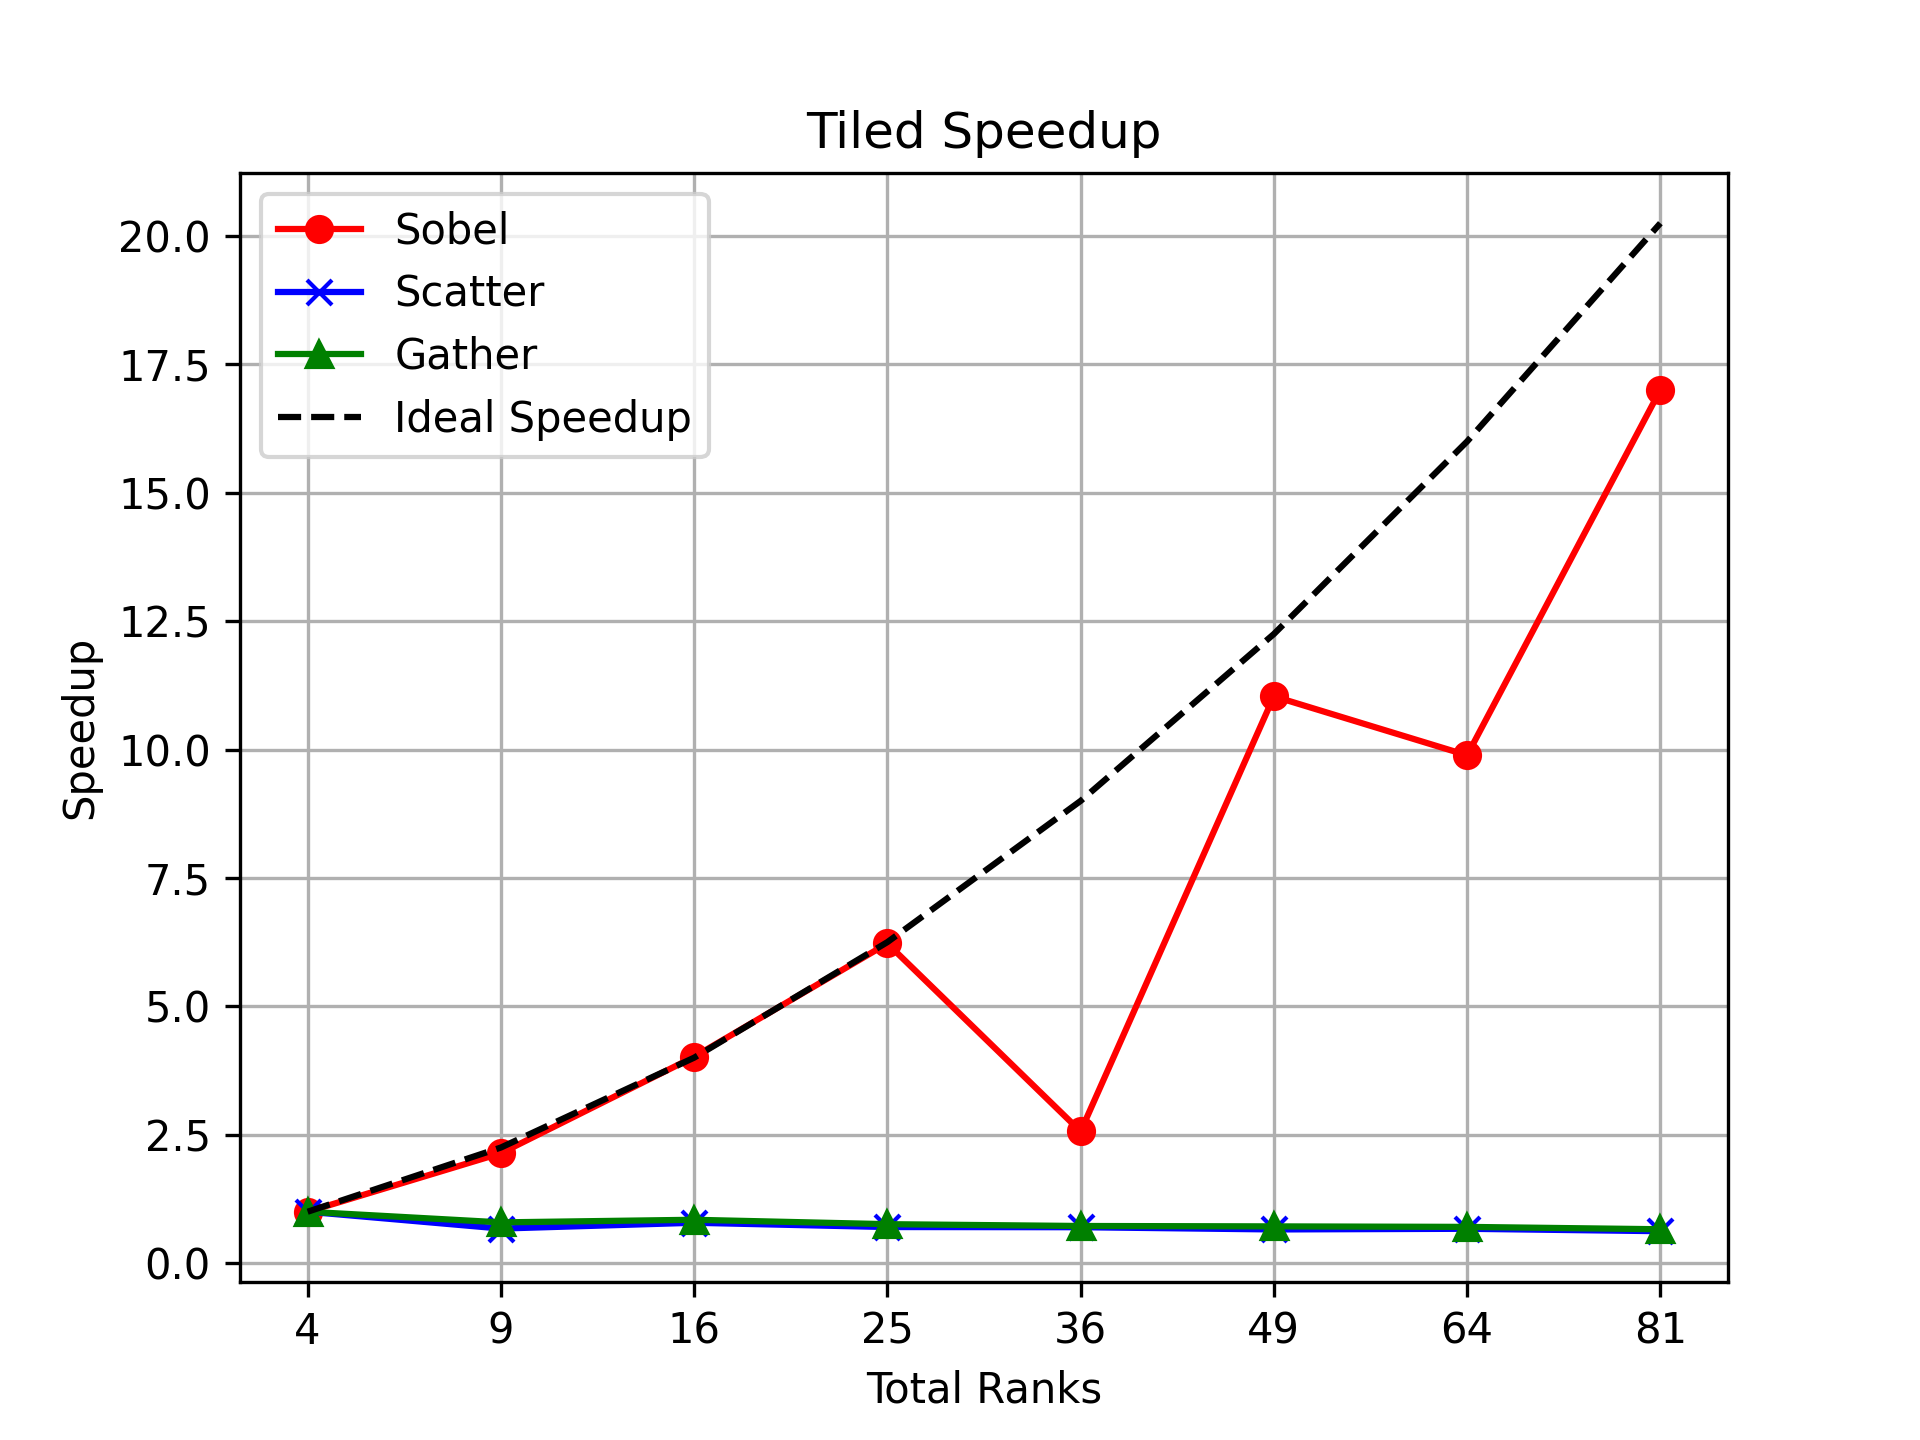
\includegraphics[width=1.0\linewidth]{images/tiled_speedup.png}
    \caption{Speedup chart for Tiled decomposition.}
    \label{fig:speedup-tiled}
\end{figure}

In this section, we analyze the runtime performance of the Sobel filter using three grid decomposition strategies: Column-slab, Row-slab, and Tiled decomposition. The speedup charts for these strategies, shown in Figures~\ref{fig:speedup-column},~\ref{fig:speedup-row}, and~\ref{fig:speedup-tiled}, illustrate the speedup of runtimes for the three computational stages: scatter, process, and gather. Below, we describe the observed performance characteristics for each strategy and discuss the underlying reasons.

As shown in Figure~\ref{fig:speedup-column}, the Column-slab decomposition achieved consistent speedup up to a total rank of 49, nearing ideal performance. However, the speedup gains plateaued at a total rank of 64, and a performance degradation was observed at a total rank of 81.

In contrast, as illustrated in Figure~\ref{fig:speedup-row}, the Row-slab decomposition showed consistent speedup with increasing total ranks, although it began to deviate slightly from ideal performance starting at a total rank of 36.

As shown in Figure~\ref{fig:speedup-tiled}, the Tiled decomposition consistently achieved near-ideal speedup, maintaining strong performance up to a total rank of 64. Unlike the Column-slab, it did not exhibit performance degradation at higher ranks.

The performance behavior of the Column-slab decomposition was initially expected to outperform the others due to its narrower tile width, which enhances cache efficiency when transitioning between rows. While it did show better speedup than Row-slab for lower ranks, the unexpected performance drop at a total rank of 81 may be attributed to inherent load imbalances. For instance, as shown in Table~\ref{tab:last-grid-sizes} and \ref{tab:last-grid-sizes}, the base grid size for 64 ranks is \(111 \times 5146\), with a last tile size of \(119 \times 5146\). In contrast, the base grid size for 81 ranks is \(87 \times 5146\), with a last tile size of \(152 \times 5146\). This disparity arises because the current implementation uses fixed dimensions for all tiles except the last one, causing the last tile to be disproportionately larger. This imbalance likely limited overall performance. To address this, a more balanced tile computation scheme should be implemented to ensure uniform tile sizes.

The superior performance of the Tiled decomposition is likely due to its more evenly distributed tile sizes, which mitigate the impact of slower ranks on runtime. As the runtime is ultimately constrained by the slowest rank, reducing disparities in tile sizes directly improves performance.

\begin{table}
    \centering
    \begin{tabular}{c|c|c|c}
        \textbf{Rank} & \textbf{Column-slab} & \textbf{Row-slab} & \textbf{Tiled} \\
        \hline
        4  & 1778 x 5146& 7112 x 1286& 3556 x 2573\\
        9  & 790 x 5146& 7112 x 571& 2370 x 1715\\
        16 & 444 x 5146& 7112 x 321& 1778 x 1286\\
        25 & 284 x 5146& 7112 x 205& 1422 x 1029\\
        36 & 197 x 5146& 7112 x 142& 1185 x 857\\
        49 & 145 x 5146& 7112 x 105& 1016 x 735\\
        64 & 111 x 5146& 7112 x 80& 889 x 643\\
        81 & 87 x 5146& 7112 x 63& 790 x 571\\
    \end{tabular}
    \caption{Base grid size of the tile for each decomposition method.}
    \label{tab:base-grid-sizes}
\end{table}

\begin{table}
    \centering
    \begin{tabular}{c|c|c|c}
        \textbf{Rank} & \textbf{Column-slab} & \textbf{Row-slab} & \textbf{Tiled} \\
        \hline
        4  & 1778 x 5146& \(7112 \times 1288\) & \(3556 \times 2573\) \\
        9  & 792 x 5146& \(7112 \times 578\)  & \(2372 \times 1716\) \\
        16 & 452 x 5146& \(7112 \times 331\)  & \(1778 \times 1288\) \\
        25 & 296 x 5146& \(7112 \times 226\)  & \(1424 \times 1030\) \\
        36 & 217 x 5146& \(7112 \times 176\)  & \(1187 \times 861\)  \\
        49 & 152 x 5146& \(7112 \times 106\)  & \(1016 \times 736\)  \\
        64 & 119 x 5146& \(7112 \times 106\)  & \(889 \times 645\)   \\
        81 & 152 x 5146& \(7112 \times 106\)  & \(792 \times 578\)   \\
    \end{tabular}
    \caption{Grid size of the last tile for each decomposition method.}
    \label{tab:last-grid-sizes}
\end{table}


The scatter and gather runtimes exhibited similar performance across all decomposition strategies. While their speedup dropped by approximately 30\% when increasing the total rank from 4 to 9, the performance stabilized for higher ranks. This consistency can be attributed to the use of subarray datatypes, which optimize communication by transforming data before transmission. By sending subregions of data in a single operation instead of row-by-row transfers, the number of communication events between ranks is minimized, leading to nearly identical scatter and gather performance across all methods.

\subsection{Data Movement Performance Study}
\label{subsec:data-movement-performance-study}

In this section, we analyze the data movement performance for different grid decomposition strategies (Column-slab, Row-slab, and Tiled) in terms of the number of messages sent and the total data moved between ranks during the scatter and gather phases. Table~\ref{tab:data-movement} summarizes the number of messages and the total data moved for varying levels of concurrency.

The observed data movement is consistent across all decomposition methods due to the use of subarray data types for inter-rank communication. This approach minimizes the number of messages sent, as subarrays allow the transmission of contiguous subregions of data in a single operation rather than row-by-row communication.

\begin{table}[htbp]
    \centering
    \begin{tabular}{c|c|c|c|c|c|c} 
        \textbf{Ranks} & \multicolumn{2}{c|}{\textbf{Column-slab}} & \multicolumn{2}{c|}{\textbf{Row-slab}} & \multicolumn{2}{c}{\textbf{Tiled}} \\ 
         & \textbf{Count} & \textbf{Bytes} & \textbf{Count} & \textbf{Bytes} & \textbf{Count} & \textbf{Bytes} \\ 
        \hline
        4  & 6   & 220MB & 6   & 220MB & 6   & 220MB \\ 
        9  & 16  & 261MB & 16  & 261MB & 16  & 260MB \\ 
        16 & 30  & 275MB & 30  & 275MB & 30  & 275MB \\
        25 & 48  & 282MB & 48  & 282MB & 48  & 281MB \\
        36 & 70  & 286MB & 70  & 287MB & 70  & 285MB \\
        49 & 96  & 289MB & 96  & 290MB & 96  & 287MB \\
        64 & 126 & 291MB & 126 & 292MB & 126 & 289MB \\
        81 & 160 & 292MB & 160 & 294MB & 160 & 290MB \\ 
    \end{tabular}
    \caption{\textbf{Number of messages sent and total data moved between ranks during the scatter and gather phases.}}
    \label{tab:data-movement}
\end{table}
\FloatBarrier
\subsection{Overall Findings and Discussion}
\label{subsec:overall-findings-and-discussion}
% Subsection - overall findings and discussion. Please think about and provide comments, substantiated with the performance data you have collected, on the following issues/questions: How does the amount of data moved vary as a function of grid decomposition strategy? What changes might you make to the overall design of this code to improve the runtime performance of data movement? What might be sources of errors or inaccuracies in how we measure performance (runtime, data movement) in these studies?

The amount of data moved remains relatively consistent across decomposition strategies, likely due to the use of the subarray data type. This approach appears to achieve near-optimal data movement efficiency. To further improve the runtime performance of the Sobel operation, it is recommended to ensure that the grid size of all tiles is as evenly distributed as possible. The current approach, where all tiles have the same size except the last one, can lead to performance bottlenecks, as the overall runtime is constrained by the rank with the longest execution time.

Potential sources of errors or inaccuracies in performance measurement, particularly in runtime and data movement, include the timing methodology employed in rank 0. While using \texttt{MPI\_Barrier} ensures that all ranks complete the preceding code region before proceeding, it does not guarantee synchronization in the actual execution of subsequent operations across all ranks. This lack of strict synchronization may lead to discrepancies in the recorded execution times.



%% if specified like this the section will be committed in review mode
\acknowledgments{
This paper was edited with the assistance of \textit{ChatGPT (GPT-4o and GPT-4o with canvas)} (accessed October 2024), which was primarily used for correcting grammatical errors and rephrasing. This research was supported by resources from the National Energy Research Scientific Computing Center (NERSC), a Department of Energy Office of Science User Facility, under NERSC award DDR-ERCAP m3930 for 2024.
}

\bibliographystyle{abbrv-doi}

% uncomment the following line if you decide to include a bibliography (references) with your homework writeup
\bibliography{template}
\end{document}
